\chapter{Actividades}
\section{Introducción}
Los diagramas de actividades, junto a los de clases y casos de uso, son diagramas de comportamiento, ya que describen como funcionará ya sea de un algoritmo o incluso de un componente completo. Estos brindan grandes ventajas, como lo es mostrar un flujo de trabajo entre los usuarios y un sistema, clarificar ese tipo de procesos y traer simplificación.
Por ello, para describir cómo será el flujo de trabajo del software, se utilizarán los diagramas de actividades ya que estos permiten detallar en un lenguaje de alto nivel, los procesos que se llevan a cabo. 
\section{Marco Teórico}
Un diagrama de actividades está constituido por:
\begin{itemize}
\item Actividad: Es un comportamiento que describe una serie de acciones de forma determinada y organizada.
\begin{figure}[H]
	\centering
	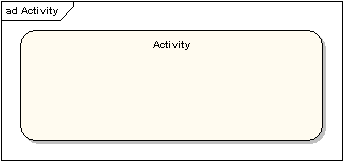
\includegraphics[width=0.5\linewidth]{diseno/actividades/imgs/1}
	\caption{Actividad. Imagen tomada de internet}
	\label{fig:gantt}
\end{figure}
\item Acción: Una acción representa un solo paso dentro de una actividad. Las acciones se denotan por rectángulos con las puntas redondeadas.
\begin{figure}[H]
	\centering
	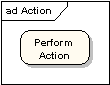
\includegraphics[width=0.5\linewidth]{diseno/actividades/imgs/3}
	\caption{Accion. Imagen tomada de internet}
	\label{fig:gantt}
\end{figure}
\item Flujo de control: Este muestra el flujo de una acción a otra. Se denota por una flecha.
\begin{figure}[H]
	\centering
	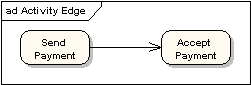
\includegraphics[width=0.5\linewidth]{diseno/actividades/imgs/2}
	\caption{Flujo de control. Imagen tomada de internet}
	\label{fig:gantt}
\end{figure}
\item Nodo inicial: Es el primer nodo, se describe por un gran punto negro.
\begin{figure}[H]
	\centering
	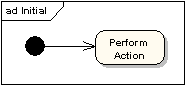
\includegraphics[width=0.5\linewidth]{diseno/actividades/imgs/6}
	\caption{Nodo inicial. Imagen tomada de internet}
	\label{fig:gantt}
\end{figure}
\item Nodo de decisión y combinación: Los nodos de decisión y combinación tienen la misma notación: una forma de diamante.  Los flujos de control que provienen de un nodo de decisión tendrán condiciones de guarda que permitirán el control para fluir si la condición de guarda se realiza.
\begin{figure}[H]
	\centering
	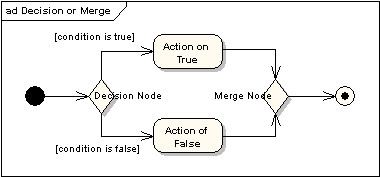
\includegraphics[width=0.5\linewidth]{diseno/actividades/imgs/4}
	\caption{Nodo de decisión y combinación. Imagen tomada de internet}
	\label{fig:gantt}
\end{figure}
\item Nodo de bifurcación y unión: Las bifurcaciones y uniones tienen la misma notación: una barra a la que llegan o de la que salen flujos de control). Estos indican el comienzo y final de hilos actuales de control.
\begin{figure}[H]
	\centering
	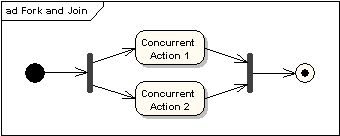
\includegraphics[width=0.5\linewidth]{diseno/actividades/imgs/5}
	\caption{Nodo de bifurcación y unión. Imagen tomada de internet}
	\label{fig:gantt}
\end{figure}
\item Particiones: 	Una partición se utiliza para separar acciones dentro de una actividad, se denota de la siguiente manera:
\begin{figure}[H]
	\centering
	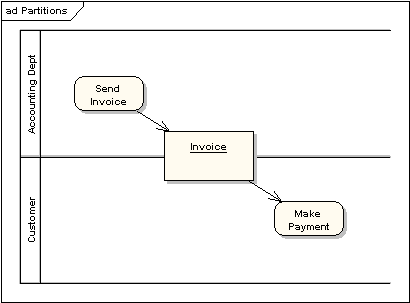
\includegraphics[width=0.5\linewidth]{diseno/actividades/imgs/7}
	\caption{Partición. Imagen tomada de internet}
	\label{fig:gantt}
\end{figure}
\end{itemize}
%http://www.sparxsystems.com.ar/resources/tutorial/uml2_activitydiagram.html
\section{Diagrama de actividades}
\begin{figure}[H]
	\centering
	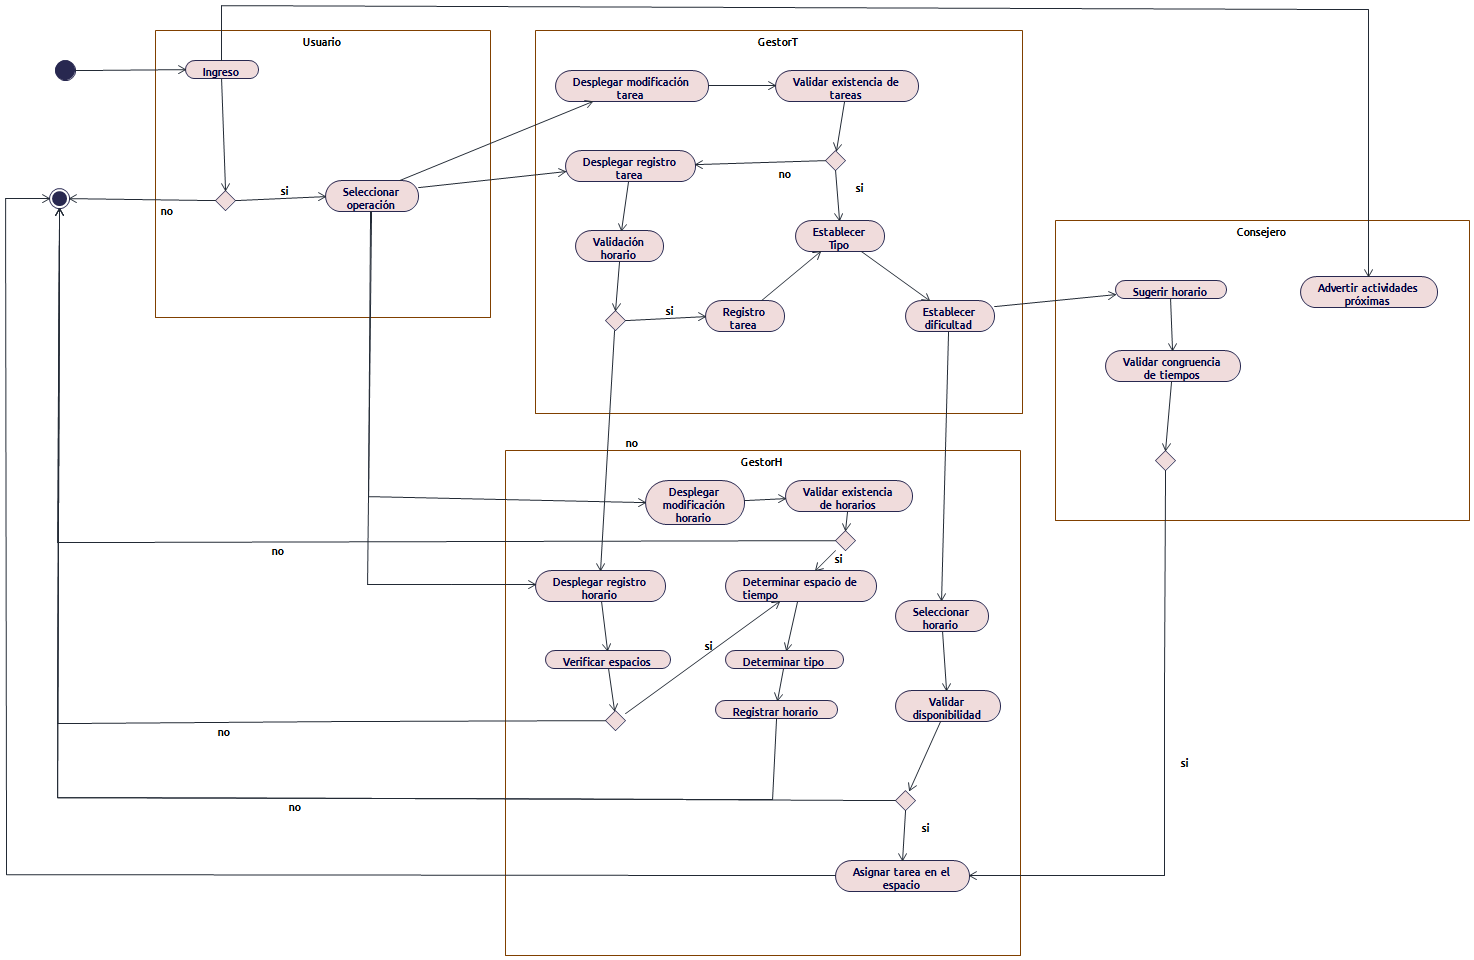
\includegraphics[width=1\linewidth]{diseno/actividades/imgs/actividades}
	\caption{Diagrama de actividades. Fuente autor.}
	\label{fig:gantt}
\end{figure}